\chapter{Tehtävä 3: Gorilla -peli \label{chap:Teht=0000E4v=0000E4-2}}

\section{Peliä kuvaavat luokkakokonaisuudet (a,b)}

\label{Peliä kuvaavat luokkakokonaisuudet (a,b)}

Kuvausten ja tehtävien pohjalta on tehty luokkakaavio kuvassa \ref{Gorilla},
jolla pyrin kuvaamaan lopullista peliä. Luokkakaaviossa on olioiden hierarkian
lisäksi kuvattu niiden määräsuhteita ja abstraktit luokat on merkitty sinisen
sijaan valkoisella pohjalla.

\begin{figure}
\centering 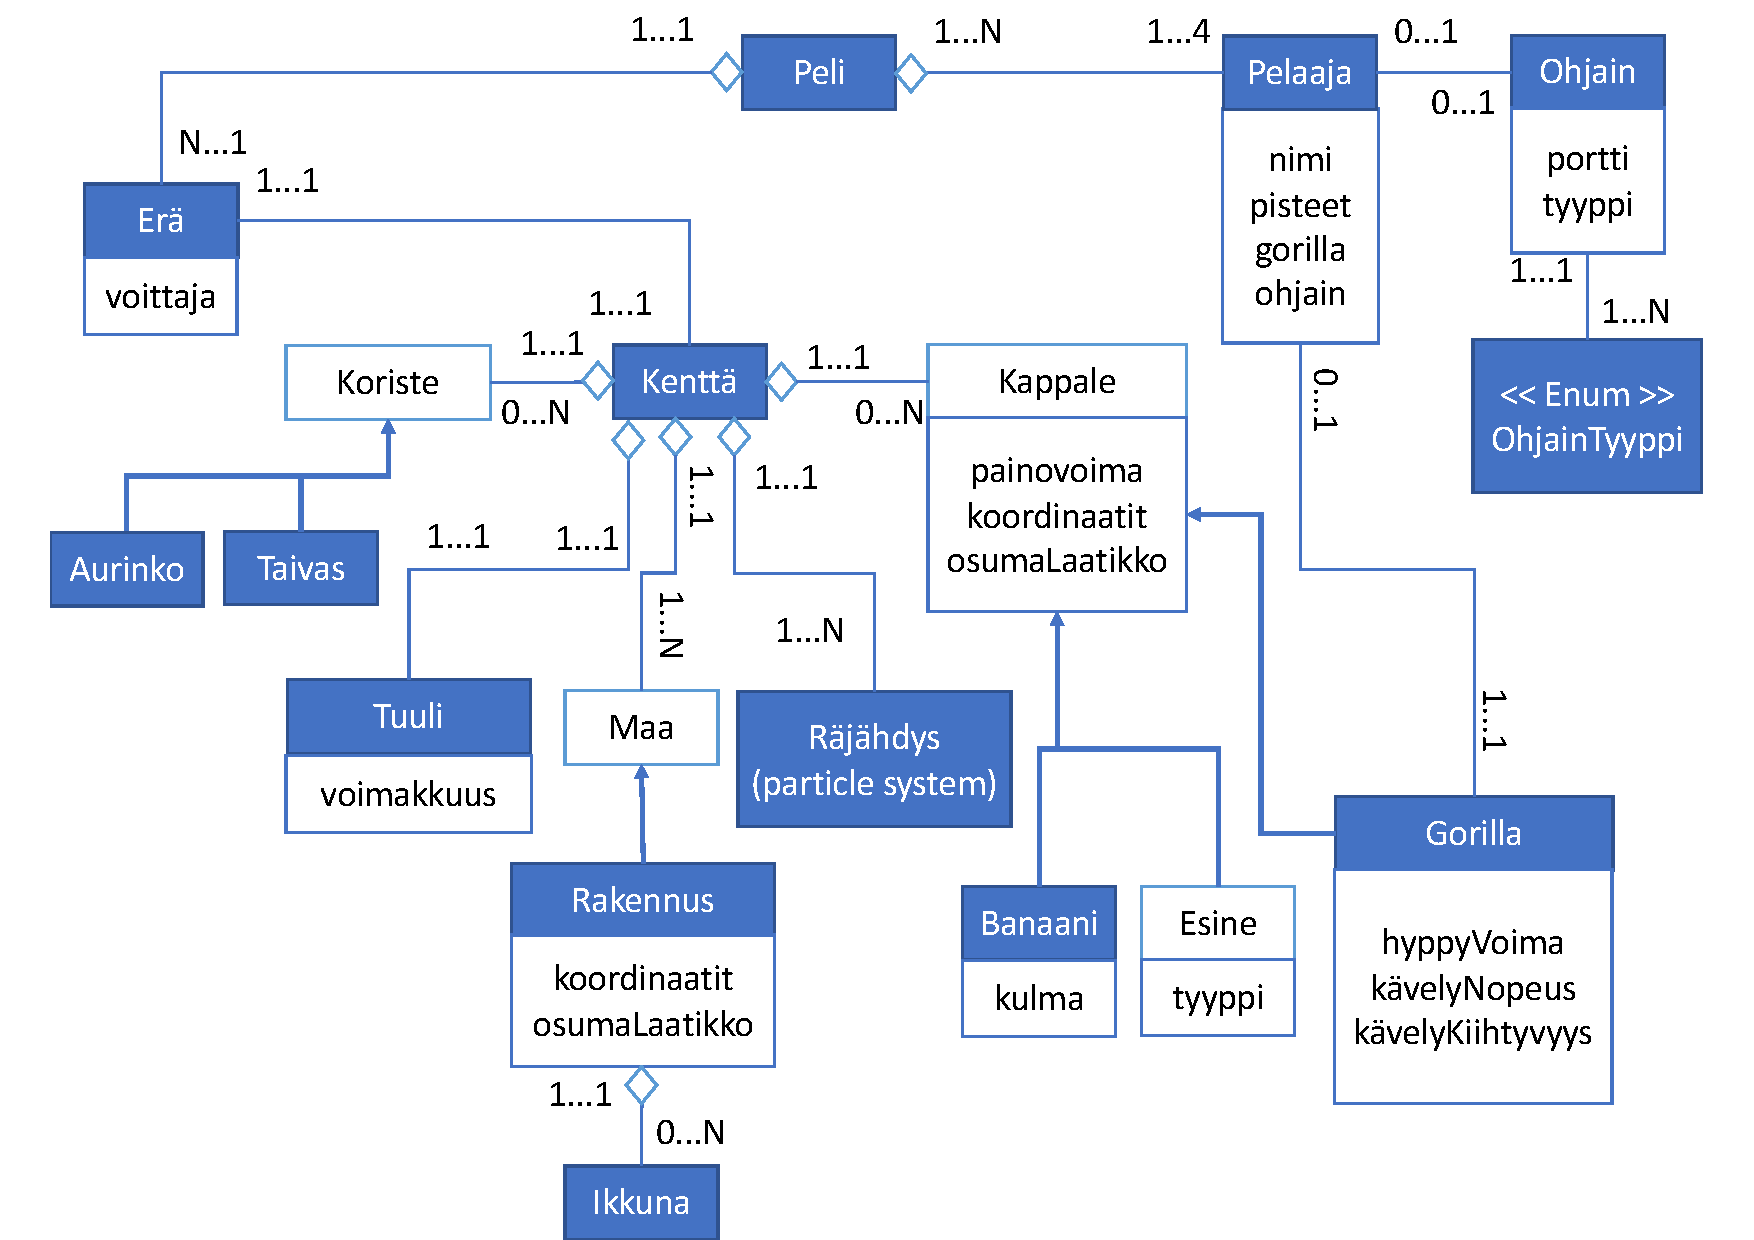
\includegraphics[width=0.5\textwidth]{kuvat/GorillaPeli}
\caption{Luokkakaavio Gorilla-Pelistä}
\label{Gorilla} 
\end{figure}

Kuvasta \ref{Gorilla} on jätetty selkeyden vuoksi merkitsemättä luokat vektori,
osumalaatikko ja rajapinnat aktiivinen, piirrettävä, heitettävä ja kerättävä.
Nämä kaikki luokat voidaan jakaa suunnittelu, analyysi ja toteutusluokkiin (kts
\ref{Gorillajako}), jossa suunnitteluluokkiin kuuluu pääasiassa abstrakteja
luokkia. Analyysiluokista löytyy pelin rakenteeseen liittyviä luokkia ja
tuuli-luokka jota ei ruudulla suoraan näe vaan liittyy enemmän pelimoottorin
toimintaan.

\begin{figure}
\centering 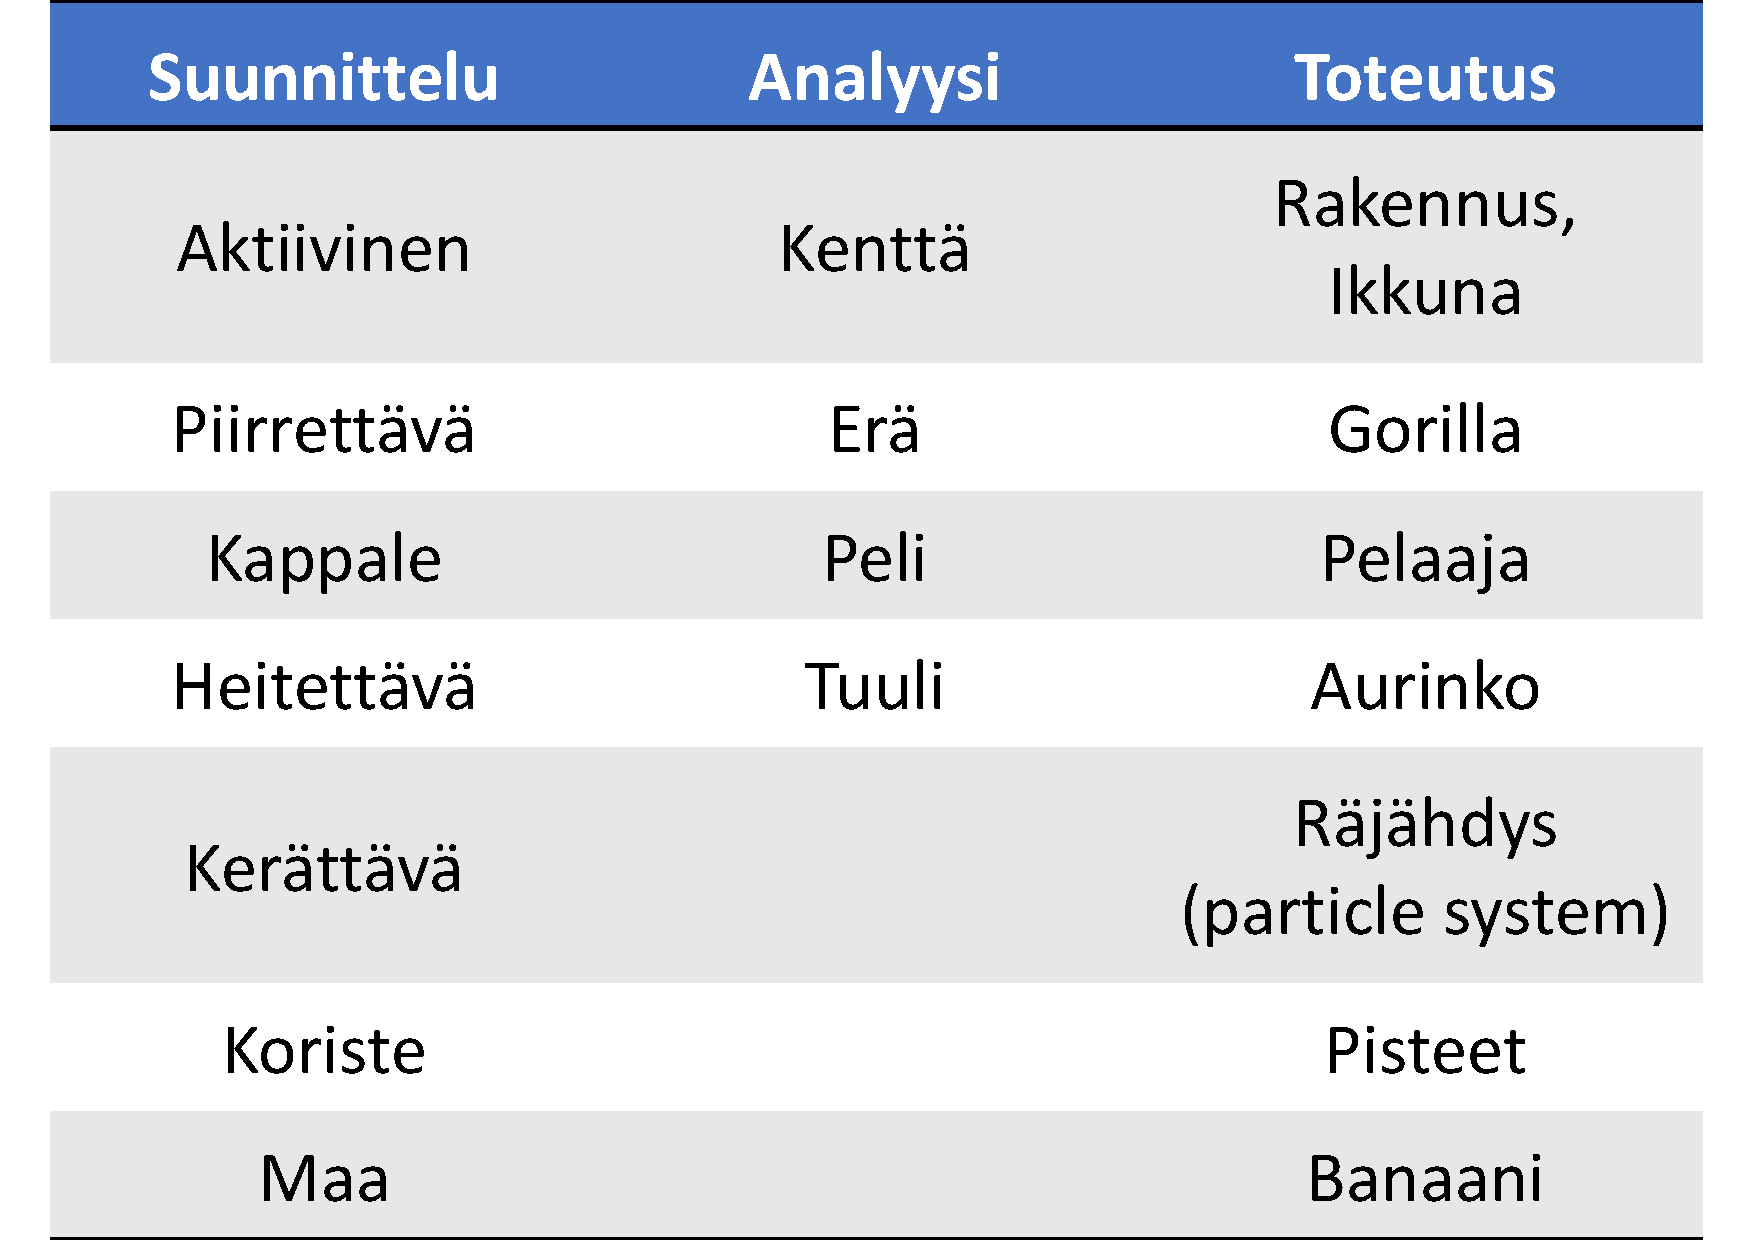
\includegraphics[width=0.5\textwidth]{kuvat/GorillaLuokat}
\caption{Suunnittelu-, analyysi ja toteutusluokkiin jako}
\label{Gorillajako} 
\end{figure}

Toteutusluokista löytyy selkeitä käsitteitä, joita pelissä nähdään visuaalisina
elementteinä ja näitä näkyviä olioita yhdistää myös rajapinta Piirrettävä, joka
määrittelee millaiset metodit tulee luokasta löytyä, että se voidaan piirtää
ruudulle. Aktiivisten luokkien oliot ovat sellaisia, joille löytyy oma
päivitysmetodi mikä toteutetaan jokaisen tick() -metodin tai toisin sanoen
jokaisen pelin päivitysiteraation aikana. 

Esineet ovat kerättäviä asioita pelikentiltä, jotka voisivat olla esimerkiksi
pisteitä, lisä elämiä tai banaaneja, joita voi heitellä toisten pelaajien niskaan. Itse rajapinta
Heitettävä kuvaa kaikkia olioita, joita pelaaja voi singota omalla gorillallaan.
Nämä kaikki rajapinnat kuvaavat pelissä tapahtuvia vuorovaikuttavia elementtejä,
mutta sen lisäksi tarvitaan koristeita, jotka tuovat pelin taustaksi grafiikkaa
ja mallintavat selkeästi pelaajalle missä rakennukset peliruudulla ovat.

\section{Pakettikokonaisuudet ja uudelleenkäytettävyys (c, d)}

\label{Pakettikokonaisuudet ja uudelleenkäytettävyys (c, d)}

Kuvan \ref{Gorilla} luokkia voidaan jakaa ryhmiin, jotka kuvaavat
pääsääntöisesti jotain pelin osa-aluetta niin, että vuorovaikutukset ryhmän
sisällä on suurempaa kuin ryhmien välillä. Ryhmät voitaisiin nimetä paketeiksi
seuraavalla tavalla:

\begin{itemize}
\item \underline{Player} (\underline{Pelaaja}, \underline{Ohjain})
\item \underline{Engine} (\underline{Kenttä}, \underline{Kappale},
\underline{Maa}, \underline{Esine})
\item Map (Rakennus, Ikkuna)
\item Character (Banaani, Gorilla)
\item Graphics (Aurinko, Taivas)
\item \underline{Menu} (\underline{Peli})
\end{itemize}

Player-paketissa olisi työkaluja pelaajien ja pelaajien käyttämien ohjainten
hallintaan. Engineä pystytään uudelleenkäyttämään, kun halutaan tehdä
samanlaiseen pelimekaniikkaan liittyvä peli tai modi. Menu-pakettilla voidaan
muodostaa toinen moninpeli, jossa 1-4 pelaajaa kamppailee toisiaan vastaan
erissä, joiden pisteitä lasketaan. Map, Character, Graphics paketit liittyvät
tiiviisti pelin ulkonäköön ja olemukseen, joten muita pelejä tehdessä näitä
paketteja tuskin pystyy paljon käyttämään hyväksi.

\section{Fysiikan mallinnuksen soveltaminen (e)}

\label{Fysiikan mallinnuksen soveltaminen (e)}

Fysiikanmallinnuksen soveltaminen pelimoottoriin voidaan tehdä monella tavalla
ja se riippuu pääsääntöisesti pelistä. Joissain arcade -peleissä fysiikan lakeja
halutaan venyttää ja muokata niin, että pelikokemus on viihdyttävämpi. Tässä
tapauksessa voimille ja kentille voi tehdä omat oliot, jolloin pelin logiikan
kehityksessä näitä voimia tai impulsseja voidaan säätää yliampuviksi tarpeen
mukaan.

Jos pelissä on kyseessä enemmän simulointi, jossa halutaan, että samat fysiikan
lait pätevät kaikkialla pelikentällä kaikille olioille, niin esimerkiksi
Painovoima, Voima ja Impulssi -olioiden tekeminen on turhaa. Fysiikan lait
pystytään silloin kuvaamaan esimerkiksi kuvan \ref{Gorilla} kaltaisessa
luokkahierarkiassa pelkästään Kappale -luokan sisällä, jolloin yksikään
aliluokka tai olio ei pysty tästä säännöstä poikkeamaan.

Esimerkiksi painovoiman, tai pikemminkin normaalikiihtyvyyden suuruus voitaisiin
määrätä final static -muodossa vektoriksi, jolloin kaikki kappaleet pelissä
joutuisivat sitä noudattamaan. Normaalikiihtyvyyden vektori kannattaisi pitää
vähintään static -muotoisena, jolloin jos maan painovoimakentästä siirryttäisiin
kuun painovoimaan, niin kaikki pelialueen oliot välittömästi päivittyisivät
tähän. Pelimoottori ei näytä välttämättä eheältä, jos jotkin kappaleet liikkuvat
kuin `eri planeetalla`.

Voima tai Painovoima -luokista luopuminen ei kumminkaan tarkoita sitä, että
pelimoottorin mekaniikan toteuttavissa metodeissa nämä käsitteet ei tarvitsisi
olla hyvin dokumentoituja. Päinvastoin: metodien toteutuksessa tulee nimetä
hyvin selkeästi milloin on kyse kiihtyvyydestä, milloin voimasta tai milloin
liiketilasta. Dokumentaatiossa kannattaa myös merkitä, että mikä rivi toteuttaa
minkäkin fysiikan lain: Newtonin lait, Galileon suhteellisuus, voimien
resultanttivektorin summaus ja jotta fysiikan mallinnuksen tuottava algoritmi on
selkeästi luettavissa.

Tekijänä Pasi Toivanen (517487)
